\section{Simulador}
\label{cap:simulador}

O objetivo da simulação é permitir testes em ambiente controlado, 
de forma a se averiguar a precisão, acurácia e velocidade de processamento da posição por parte do Star Tracker. 
Para isto, a simulação implementa modelos matemáticos que representem o sistema real o mais fielmente possível. 

O programa foi desenvolvido de forma a permitir ao leitor testar diferentes cenários de forma rápida e intuitiva,
podendo assim carregar diferentes arquivos como figuração de câmera, diferentes arquivos de dados de estrelas. 
Além disto, o simulador permite a visualização tanto em 3D como em 2D, para que o usuário possa ter uma visão mais clara do que está acontecendo.
A visualização em 2D permite se comparar os resultados com os resultados obtidos em outros trabalhos.

Atualmente, o simulador apenas salva o frame desejado em um arquivo de imagem, porém, o sistema foi construído a permitir a visualização em um segundo monitor do simulação em tempo real.
Isto permitirá possíveis fases de simulações com hardware real, como pode ser visto na Figura ~\ref{fig:Simulador_top} e na Figura ~\ref{fig:Simulador_tipo_meu}.

\begin{figure}[H]
    \centering
    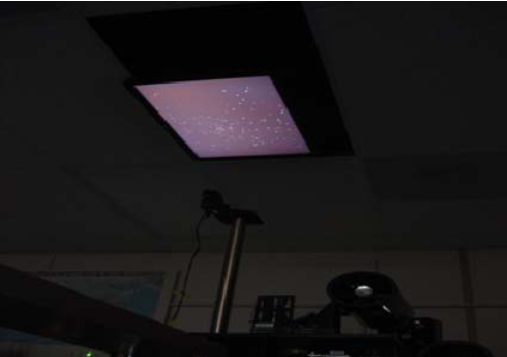
\includegraphics[width=.65\columnwidth]{images/Simulador_top.png}
    \caption{Simulação em projetor, Fonte ~\cite[]{Tappe}}
    \label{fig:Simulador_top}
\end{figure}

\begin{figure}[H]
    \centering
    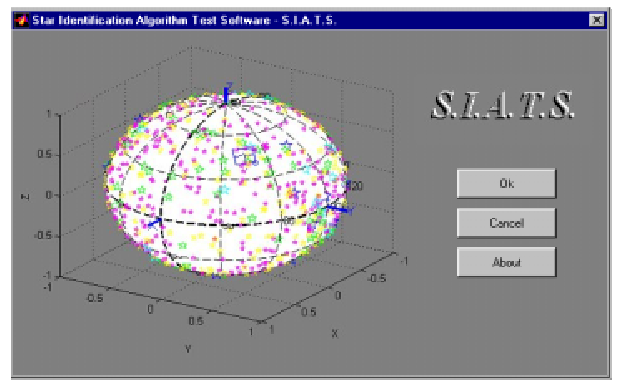
\includegraphics[width=.65\columnwidth]{images/Simulador_tipo_meu.png}
    \caption{Meu do simulador, Fonte ~\cite[]{Carvalho}}
    \label{fig:Simulador_tipo_meu}
\end{figure}

\subsection{Recursos e características}

\textbf{GUI (\textit{Graphical User Interface}):} A simulação é controlada através de uma GUI criada para facilitar o controle e a execução dos testes, também é utilizada para facilitar a visualização e a correção de possíveis erros e \textit{bugs} no software e no desenvolvimento do trabalho em geral. 
A implementação dos módulos de funcionamento do software segue conceitos dos TDD (\textit{Test driven  development}), 
juntamente da arquitetura de software MVC (\textit{model view controller}), 
para organizar o funcionamento da interface em si ~\cite[]{Martin_Fitzpatrick}.

\textbf{Gerador de campo de visão:} Esta é a função principal do software de simulação, 
que é gerar uma janela com o campo de visão que teoricamente seria visto pela câmera, 
a imagem gerada é monocromática com as estrelas projetadas sobre a superfície plana do monitor. 
Neste trabalho as estrelas simuladas são apenas círculos brancos em um fundo preto, porém são estrelas retiradas de uma base de dados reais.

\textbf{Carregamento de arquivos:} Para facilitar a mudança de parâmetros durante os testes e simulações , o software carrega todas as informações inerentes a configuração e execução dos testes, através de caixas de diálogo que pedem a seleção dos arquivos de simulação. Para uma maior modularidade, cada informação está dividida em arquivos diferentes, com arquivos separados para configuração de câmera, base de dados de estrelas e sequência de movimentos a ser realizada.

\textbf{Elementos auxiliares de visualização:} Além das funcionalidades básicas, o software implementa  recursos de configuração  de aspectos visuais. Apesar de não serem estritamente necessários são de extrema importância  para análises menos rigorosas das informações, como por exemplo, o plot 3D, a projeção cartográfica em 2D. Com opções de visualização da posição das câmeras e demais auxílios.

\textbf{Controles manuais e automáticos:} O software possui controles manuais de rotação, que permitem a rotação da simulação em todos os 3 eixos de liberdade, através de configurações na GUI, além disto o usuário pode preparar uma sequência de movimentos e suas respectivas durações previamente.

\textbf{Salvar frames:} O usuário pode salvar frames de imagem em arquivos png para facilitar a utilização posterior da posição.

\subsection{Projeção em perspectiva}

A projeção descreve matemática como representar um ponto com 3 graus de liberdade, no espaço bidimensional do monitor e do frame da câmera. Essa transformação pode ser realizada através de matrizes, que levam em consideração elementos como o ângulo focal da lente, a resolução e proporção da imagem.

\subsection{\textit{Square Frustum}}

\textit{Frustum} retangular é um espaço que contém a linha de visão de  um visualizador como se este possuísse um ângulo de visão retangular, que é caso de câmeras com CCD retangulares, para melhor entender este conceito recomenda-se a observação da Figura \ref{fig:frustum}.

\begin{figure}[H]
    \centering
    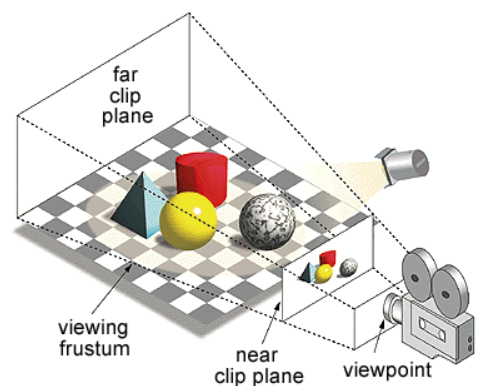
\includegraphics[width=0.5\textwidth]{images/frustum.png}
    \caption{Visualização Frustum rectangular, Fonte: ~\cite[]{the_free_dictionary}}
    \label{fig:frustum}
\end{figure}

A existência de um plano ao fundo na cena (\textit{far clip}), 
se deve ao equacionamento que leva os pontos presentes na cena 3D para o frame 2D da câmara, 
com adição do \textit{far clip} o custo de processamento requerido pelo programa diminui, 
desta forma sendo necessário equacionamento do frame da câmera, apesar deste conceito não existir em cameras reais.

Neste trabalho, convencionou-se que o ângulo de visão da câmera esteja apontado para o positivo do eixo x, 
como é mostrado na Figura \ref{fig:posicao_inicial_camera}.

\begin{figure}[H]
    \centering
    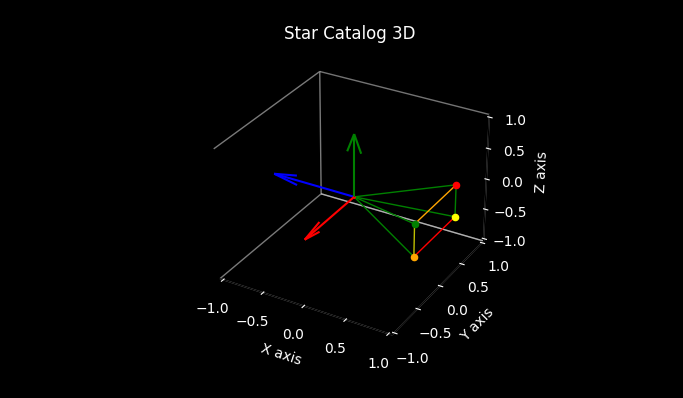
\includegraphics[width=0.5\textwidth]{images/posicao_inicial_camera.png}
    \caption{Visualização da câmera na posição inicial}
    \label{fig:posicao_inicial_camera}
\end{figure}

As setas coloridas presentes na imagem representam as coordenadas do frame da câmera, 
que seguem um esquema de cores usual para esse tipo de aplicação, 
na Figura \ref{fig:coordenadas} é demonstrado as relações X,Y e Z com as cores:

\begin{figure}[H]
    \centering
    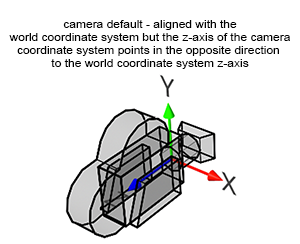
\includegraphics[width=0.5\textwidth]{images/coordenadas.png}
    \caption{Coordenadas do frame da camera. Fonte: ~\cite[]{the_free_dictionary}}
    \label{fig:coordenadas}
\end{figure}


Com isso, se desenvolveu a seguinte equação matricial da câmera, 
seguindo os passos mostrados por Brendan Galea em seu video ~\cite[]{Galea}:

\begin{equation}
    \begin{bmatrix}
        x' \\
        y' \\
        z' \\
        w
    \end{bmatrix}
    =
    \begin{bmatrix}
        \frac{f+n}{f-n} & 0                                 & 0                               & \frac{-2fn}{f-n} \\
        0               & \frac{h}{w*tan(\frac{\theta}{2})} & 0                               & 0                \\
        0               & 0                                 & \frac{1}{tan(\frac{\theta}{2})} & 0                \\
        1               & 0                                 & 0                               & 0
    \end{bmatrix}
    \begin{bmatrix}
        x \\
        y \\
        z \\
        1
    \end{bmatrix}.
\end{equation}

Em que, \textbf{f} é a distância do \textit{far plane} ao ponto (0,0,0), 
que neste caso é sempre unitário já que a estrelas estão presentes em um círculo unitário, $\Theta$ é o ângulo de abertura  da câmera, \textbf{w} é a quantidade de pixels na horizontal camera, \textbf{h} é quatidade e pixel na vertical da câmera por fim \textbf{n} é a distância do near plane, que neste caso é o coseno de $\frac{\Theta}{2}$.

Nota-se que a matriz de transformação da câmera é uma matriz 4X4 isso ocorre pois as equações de transformação são realizadas através de coordenadas homogêneas e não coordenadas cartesianas tradicionais.

Além da matriz, existe uma equação de \textit{clipping} que determina se uma estrela deve ou não aparecer no frame. 
Devido a simplicidade da simulação implementada nesse trabalho, 
essa equação se tornou apenas uma verificação se a estrela se encontrava na metade da esfera celeste em que x é positivo.

O resultado dessa simulação pode ser visto na Figura \ref{fig:resultado_simulacao}.

\begin{figure}[H]
    \centering
    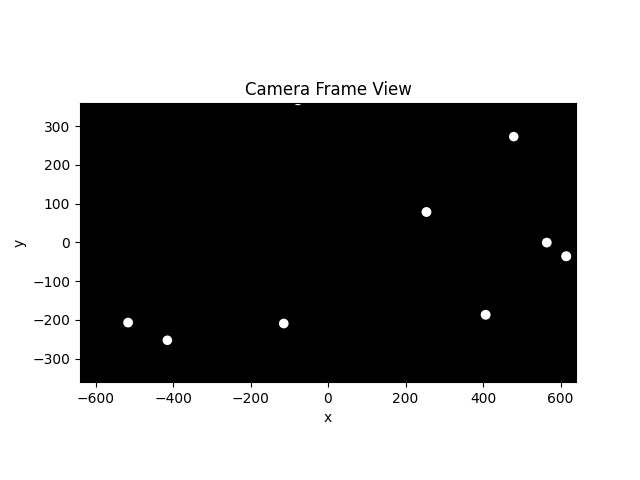
\includegraphics[width=\textwidth]{images/resultado_simulacao.png}
    \caption{Camera frame at position,declination 0º, ascensão 0º, roll 0º. Fonte: Autoria própria}
    \label{fig:resultado_simulacao}
\end{figure}

\subsection{Configurações de câmera}

No simulador, o leitor pode carregar um arquivo de câmera, que é um arquivo json, com as seguintes informações:

\begin{itemize}
    \item \textbf{ang}: Abertura da lente, nas figuras ~\ref{fig:Camera_ang_30} e ~\ref{fig:Camera_ang_20} ve-se o impacto dessa variável;\tabularnewline
    \item \textbf{w}: Quantidade de pixels que a câmera possui de altura;\tabularnewline
    \item \textbf{h}: Quantidade de pixels que a câmera possui de largura;\tabularnewline
\end{itemize}

Neste trabalho, a altura e a largura em pixel são apenas utilizadas para calcular a proporção do frame gerado, com o angulo de abertura da lente, responsável por controlar o tamanho geral do FOV da câmera.

\begin{figure}[H]
    \centering
    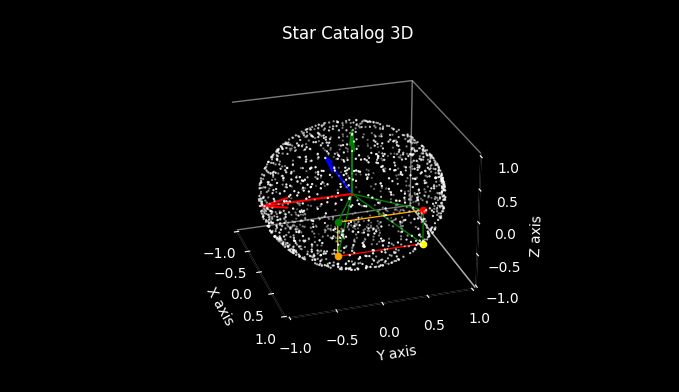
\includegraphics[width=1\columnwidth]{images/Camera_ang_30.png}
    \caption{Camera ang 30}
    \label{fig:Camera_ang_30. Fonte: Autoria própria}
\end{figure}

\begin{figure}[H]
    \centering
    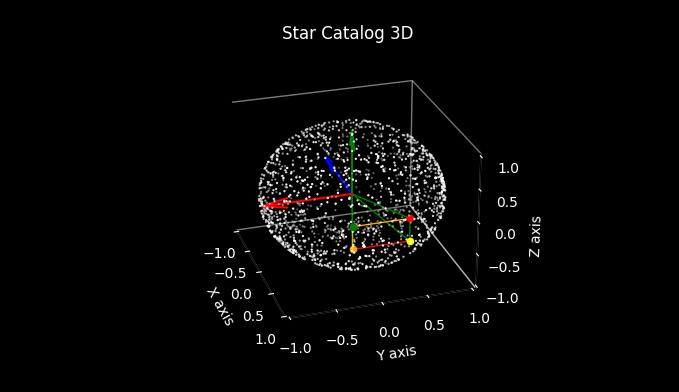
\includegraphics[width=1\columnwidth]{images/Camera_ang_20.png}
    \caption{Camera ang 20}
    \label{fig:Camera_ang_20. Fonte: Autoria própria}
\end{figure}

\section{Arquivo de estrelas}

A estrutura desse arquivo ja foi explicada na seção \ref{sec:catalogo_de_estrelas}. 
Nas figuras ~\ref{fig:my_3D} e ~\ref{fig:my_2D} são apresentados os resultados do carregamento do catalogo NASA I/239, 
filtrado para estrelas com magnitude menor que 5.

\begin{figure}[H]
    \centering
    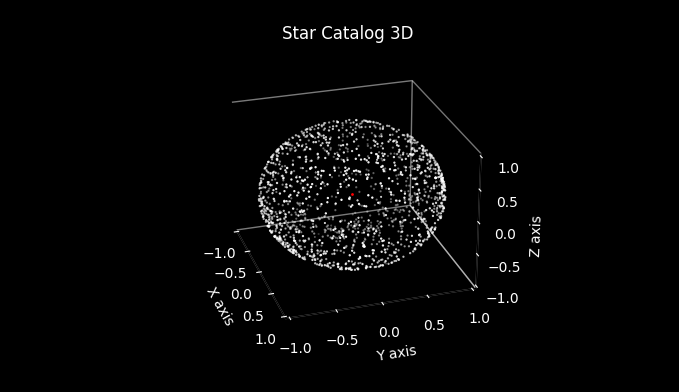
\includegraphics[width=1\columnwidth]{images/my_3D.png}
    \caption{Simulação em 3D, Fonte: Autoria própria}
    \label{fig:my_3D}
\end{figure}

\begin{figure}[H]
    \centering
    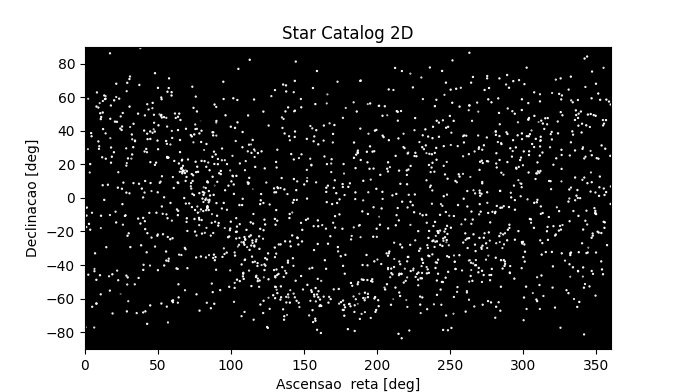
\includegraphics[width=1\columnwidth]{images/my_2D.png}
    \caption{Simulação em 2D, Fonte: Autoria própria}
    \label{fig:my_2D}
\end{figure}

Os resultados foram muito semelhantes aos obtidos por ~\cite[]{Diaz}, 
fato que corrobora a correta leitura dos arquivos de dados.
